\documentclass{article}
\usepackage[utf8]{inputenc}
\usepackage{graphicx}
\usepackage{sectsty}


\title{Game Design Document}
\author{Group 4: Pico Bello B.V.}
\date{27-11-2014}


\begin{document}
	\fontencoding{T1}\fontfamily{cmss}\fontseries{m}\selectfont

	\allsectionsfont{\fontfamily{lmss}\selectfont}


	\maketitle
	\begin{figure}[ht!]
		\centering
		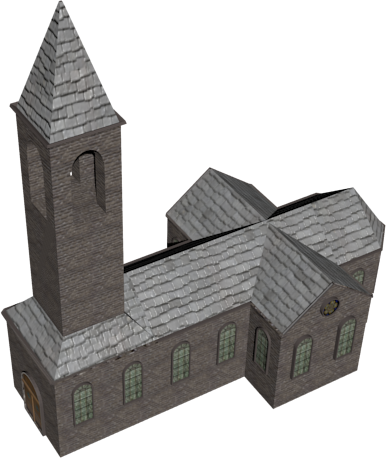
\includegraphics[width=100mm]{images/Front.png}
	\end{figure}
	\newpage
\subsection*{Project Name}
	\qquad Awesome Spel
\subsection*{Team Name}
	\qquad Group 4: Pico Bello B.V.
\subsection*{Team Members}
	\begin{itemize}
		\item \textbf{Thomas de Boer}, Game Designer
		\item \textbf{Luuk de Niet}, Lead Artist
		\item \textbf{Boyd Verdoorn}, Lead Programmer
		\item \textbf{Rense Wisse}, World Builder
		\item \textbf{Jesper Spillenaar Bilgen}, Producer
	\end{itemize}

	\newpage

\section{Introduction}
	Awesome Spel is a game that is based around the old Film Noir movie genre, but with a modern twist. The game will be in color, albeit a bit grimey. The player should solve a hideous murder, while playing as a detective, George Carter. There are several ways to collect evidence, by searching for clues, interrogation and exploration.

	\subsection{Inspiration}
		Our Inspiration was games such as LA noire, Ace Attorney and The Walking Dead, story based exploration games, where the outcome changes depending on the choices made by the player.\\
		The orthographic platform styled level design was inspired by bastion and similar games.\\
		The art style and setting are mostly inspired by Bioshock Infinite and the movie Blade Runner.
\section{Target Audience}
	\begin{itemize}
		\item Male
		\item 16 to 25 years old
		\item Likes Games
		\item Likes TV Series
		\item Uses the Steam Platform
		\item Casual Gamer
	\end{itemize}
	We are targeting casual to midrange gamers, who are interested in an story based interactive experience. Because our game relies quite a bit on story, it can pique the interest of people who watch a lot of series. The age group is Teen to Young Adult, because some of the themes may not be suitable for younger children. Although we target young males, we think our game has aspects that will appeal to a larger audience.


\section{Platform \& Controls}
	The game is developed for PC, with mac as a possible addition. We use the mouse and keyboard as control devices, because the mouse has the ability to precisely point at objects. This gives the player more control over the game.

\section{Story, Characters and setting of the game}

\section{Artificial Intelligence}
	We use A* to enable our Non Player Characters to wander around the city. 

\section{Level \& Environment Design}
	There are two basic level types in this game. The city and individual rooms.
	\subsection{City}
		We have a single city we can walk through and find hidden clues. The city is basically one large map with roads and buildings. On this map there are several landmarks, a church in a small park, the police station, a hotel and a hospital. The player is free to roam this city. The city is procedurally generated. The camera is fixed to the player in a classic orthographic configuration
	\subsection{Indoors}
		These are individual rooms where the player can go to via the landmarks or events. We will create several rooms, such as: The murder scene, a hotel room, the police chiefs office, the inside of the church etc. In these rooms there are clues to be found. The player can walk and click objects that may be clues.

\section{Gameplay \& Mechanics}

\section{Art}
	\subsection{Atmosphere}
		The game has a dark and gritty atmosphere.

\section{Sound of Music}

\section{User interface \& Game controls}

\end{document}